\chapter{Methodology}
\label{cp:Methodology}

  The proposed framework uses a bottom-up pipeline to 
gradually infer a high-level representation of the scratchs and stains from low-level features in an back cover of mobile phone image. Firstly by mean of wavelet transform, the surface texture properties such as scratch and stain are decomposed into so-called wavelet characteristics. Then multivariate statistical approach, i.e. Hotelling $T^{2}$ control chart is utilized to monitor the mean vector of a multivariate process, which can be used to judge the existence of scratch defects in the sample image. 

\section{Maximal variance of moving window}
For the surface of back cover of handy, we assume that the the pixels of back cover are homogeneous. Therefore, we thought of using the variance of pixel value to extract some features to represent the surface state. \\

The control charts are used spatially by moving a mask (or window) across the image and then calculating and plotting a statistic each time the mask is moved. The size of the mask depends on the expected size of the defects to be detected, with smaller defective regions requiring smaller mask sizes.~\cite{megahed2011review}

Inspired by this view, we move a 10 x 10 window across the image and calculate the variance of the pixel value each time the window is moved. Then value with the largest variance in this image is taken as the desired statistic describing this image.

\section{Wavelet transform decomposition}
  The continuous wavelet transform was computed by changing the scale of the analysis window, shifting the window in time, multiplying by the signal, and integrating over all times. In the discrete case, filters of different cutoff frequencies are used to analyze the signal at different scales. The signal is passed through a series of high pass filters to analyze the high frequencies, and it is passed through a series of low pass filters to analyze the low frequencies.~\cite{polikarTHE WAVELET TUTORIALusing}



Here is one example demonstrated by Fig.~\ref{fig:cnn} that adapted from~\cite{hijazi2015using}. 

\begin{figure}[h]
\centering
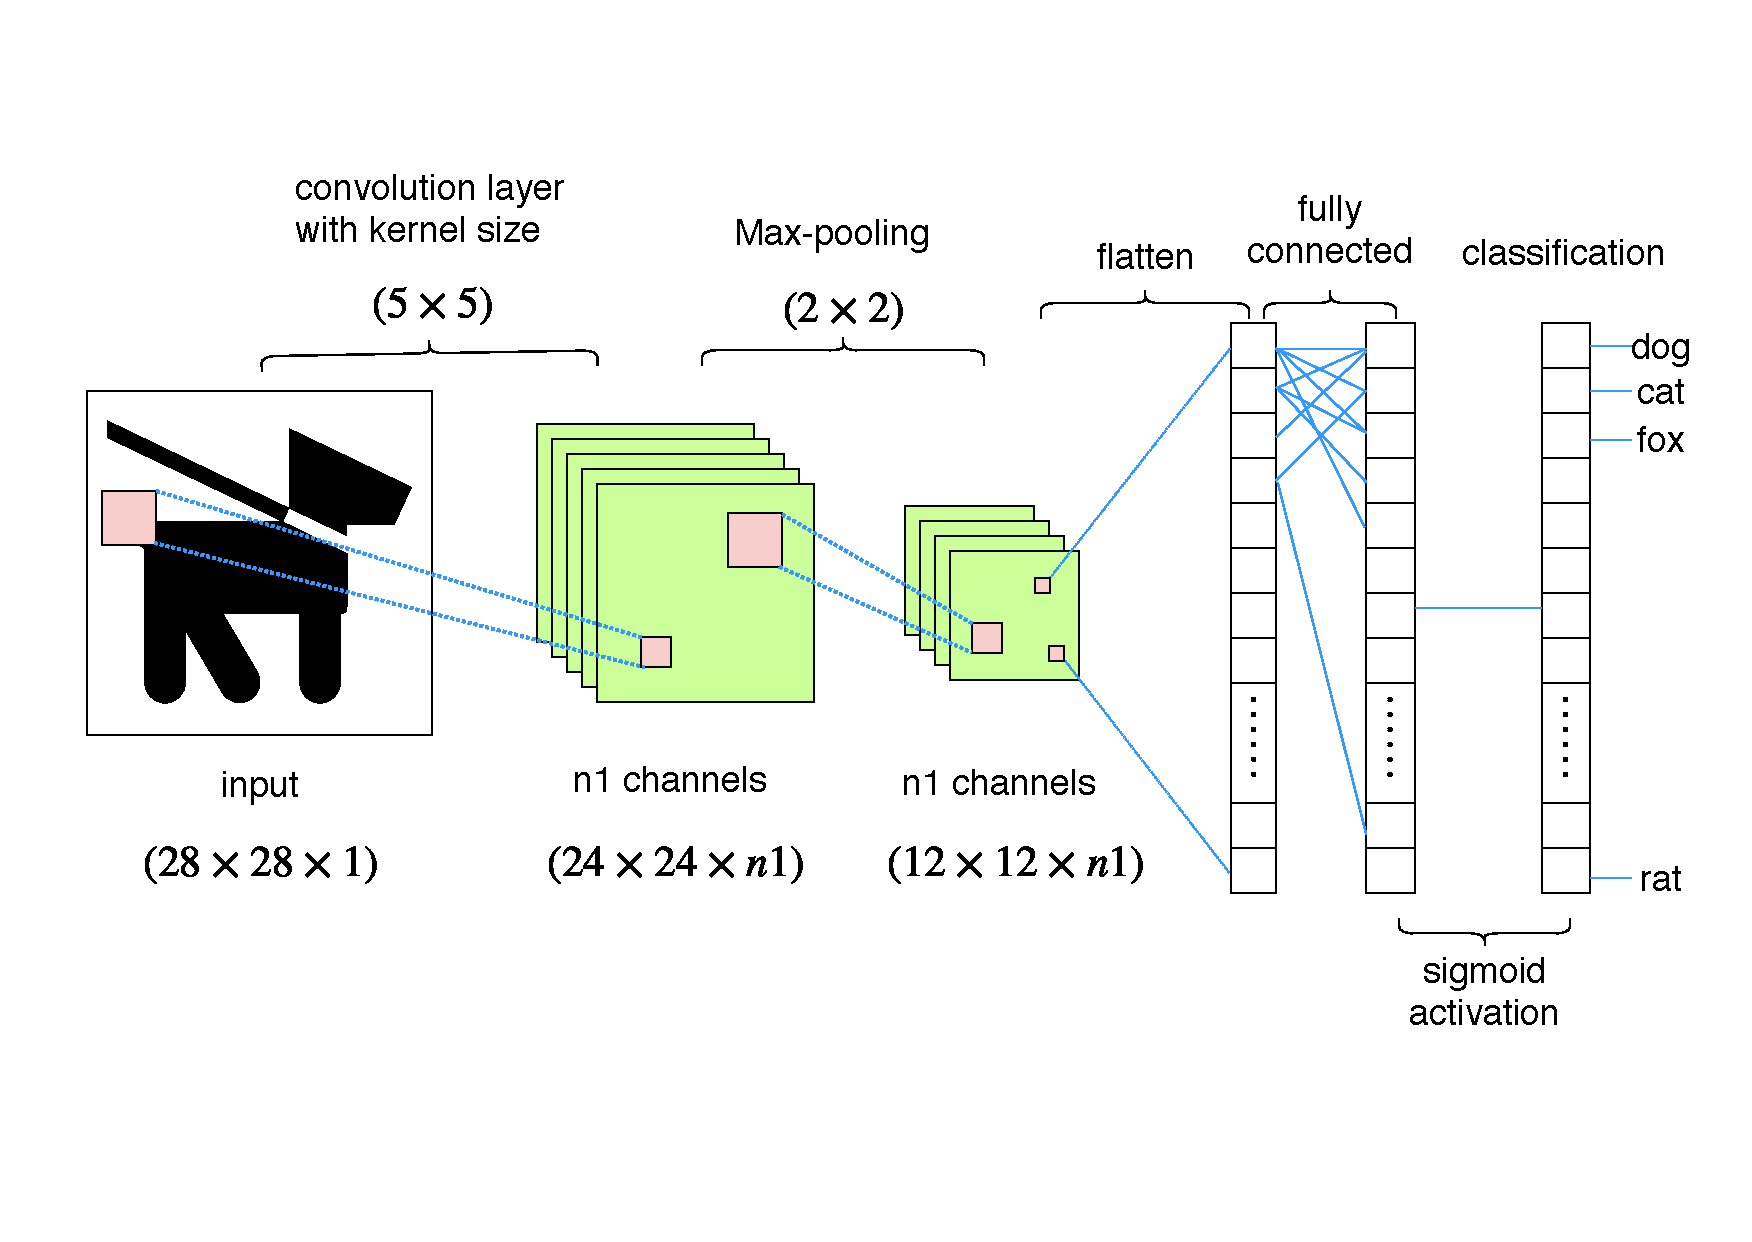
\includegraphics[width=1\textwidth]{images/cnn.pdf}
\caption[Structure of CNNs]{A general structure of CNNs, which is frequently used for image recognition. There are several layers such as input layer, convolutional layer, non-linear layer, pooling layer, and fully-connected layer. The pink squares indicate
the convolutional kernels. Figure is adapted from~\cite{hijazi2015using}.}
\label{fig:cnn}
\end{figure}



